%%%%%%%%%%%%%%%%%%%%%%%%%%%%%%%%%%%%%%%%%
% Masters/Doctoral Thesis 
% LaTeX Template
% Version 1.43 (17/5/14)
%
% This template has been downloaded from:
% http://www.LaTeXTemplates.com
%
% Original authors:
% Steven Gunn 
% http://users.ecs.soton.ac.uk/srg/softwaretools/document/templates/
% and
% Sunil Patel
% http://www.sunilpatel.co.uk/thesis-template/
%
% License:
% CC BY-NC-SA 3.0 (http://creativecommons.org/licenses/by-nc-sa/3.0/)
%
% Note:
% Make sure to edit document variables in the Thesis.cls file
%
%%%%%%%%%%%%%%%%%%%%%%%%%%%%%%%%%%%%%%%%%

%----------------------------------------------------------------------------------------
%	PACKAGES AND OTHER DOCUMENT CONFIGURATIONS
%----------------------------------------------------------------------------------------

\documentclass[11pt, oneside]{Thesis} % The default font size and one-sided printing (no margin offsets)

\graphicspath{{Pictures/}} % Specifies the directory where pictures are stored

\usepackage[square, numbers, comma, sort&compress]{natbib} % Use the natbib reference package - read up on this to edit the reference style; if you want text (e.g. Smith et al., 2012) for the in-text references (instead of numbers), remove 'numbers' 
\hypersetup{urlcolor=blue, colorlinks=true} % Colors hyperlinks in blue - change to black if annoying
\title{\ttitle} % Defines the thesis title - don't touch this

\begin{document}

\frontmatter % Use roman page numbering style (i, ii, iii, iv...) for the pre-content pages

\setstretch{1.3} % Line spacing of 1.3

% Define the page headers using the FancyHdr package and set up for one-sided printing
\fancyhead{} % Clears all page headers and footers
\rhead{\thepage} % Sets the right side header to show the page number
\lhead{} % Clears the left side page header

\pagestyle{fancy} % Finally, use the "fancy" page style to implement the FancyHdr headers

\newcommand{\HRule}{\rule{\linewidth}{0.5mm}} % New command to make the lines in the title page

% PDF meta-data
\hypersetup{pdftitle={\ttitle}}
\hypersetup{pdfsubject=\subjectname}
\hypersetup{pdfauthor=\authornames}
\hypersetup{pdfkeywords=\keywordnames}

%----------------------------------------------------------------------------------------
%	TITLE PAGE
%----------------------------------------------------------------------------------------

\begin{titlepage}
\begin{center}

\textsc{\LARGE \univname}\\[1.5cm] % University name
\textsc{\Large Master Thesis Preliminary Study}\\[0.5cm] % Thesis type

\HRule \\[0.4cm] % Horizontal line
{\huge \bfseries \ttitle}\\[0.4cm] % Thesis title
\HRule \\[1.5cm] % Horizontal line
 
\begin{minipage}{0.4\textwidth}
\begin{flushleft} \large
\emph{Author:}\\
{\authornames} % Author name - remove the \href bracket to remove the link
\end{flushleft}
\end{minipage}
\begin{minipage}{0.4\textwidth}
\begin{flushright} \large
\emph{Supervisor:} \\
\href{http://www.ntnu.edu/employees/michailg}{\supname} % Supervisor name - remove the \href bracket to remove the link  
\end{flushright}
\end{minipage}\\[3cm]
 
%\groupname\
\deptname\ % Research group name and department name
 
{\large \today}\\[4cm] % Date

\includegraphics{Figures/logo-ntnu.png} % University/department logo - uncomment to place it
 
\vfill
\end{center}

\end{titlepage}

%----------------------------------------------------------------------------------------
%	ABSTRACT PAGE
%----------------------------------------------------------------------------------------

\addtotoc{Abstract} % Add the "Abstract" page entry to the Contents

\abstract{\addtocontents{toc}{\vspace{1em}} % Add a gap in the Contents, for aesthetics

This page should hold the abstract. The abstract will serve both as an introduction to the paper and a summary of both the literature study and the proposed solution.
}

\clearpage % Start a new page

%----------------------------------------------------------------------------------------
%	LIST OF CONTENTS/FIGURES/TABLES PAGES
%----------------------------------------------------------------------------------------

\pagestyle{fancy} % The page style headers have been "empty" all this time, now use the "fancy" headers as defined before to bring them back

\lhead{\emph{Contents}} % Set the left side page header to "Contents"
\tableofcontents % Write out the Table of Contents

%----------------------------------------------------------------------------------------
%	THESIS CONTENT - CHAPTERS
%----------------------------------------------------------------------------------------

\mainmatter % Begin numeric (1,2,3...) page numbering

\pagestyle{fancy} % Return the page headers back to the "fancy" style

% Include the chapters of the thesis as separate files from the Chapters folder
% Uncomment the lines as you write the chapters

% Chapter 1

\chapter{Introduction}

\label{Chapter1}

\lhead{Chapter 1. \emph{Introduction}}

%----------------------------------------------------------------------------------------
%	SECTION 1
%----------------------------------------------------------------------------------------

\section{Introduction}

The goal of this paper is to plan the improvement of the existing Flora Danica application, a modifiable edu-game built on the Kivy framework\citep{Kivy}, designed for use on large multi-touch displays in informal learning situations. The paper will look into previous research and work on related topics such as edu-games, gamification, game elements, multi-touch wall displays and tabletops, and will use concepts from these areas to improve the existing application.

The first chapter provides an introduction to the paper, the existing application and edu-games in general. The second chapter explores and discusses previous work on related topics. The third chapter proposes a solution in possible extensions to the application. It also describes the planned process for conducting the user studies. The final chapter contains final discussion as well as a summary of the paper.

%----------------------------------------------------------------------------------------
%	SECTION 2
%----------------------------------------------------------------------------------------

\section{Existing application}

The existing Flora Danica application that is being extended is a Python application built partially on the Kivy framework\citep{Kivy}. We are going to focus on improving the part built on the Kivy framework, which is a simple quiz game that can be played by two players either as a team ("team mode") or against each other ("versus mode").

During the game, the players will be presented with a series of questions, each with two alternatives for the right answer. In versus mode, each player answers the question separately, touching their answer button with one finger for the first alternative and two fingers for the second alternative. In team mode, the player to the left touches their answer button for the first alternative, while the player on the right touches their button for the second alternative.

The application allows for easy switching of content, and can be and has been modified for different institutions. Examples of different implementations of the application are those of the Norwegian Deaf Museum and of the Norwegian States Archive in Trondheim.

%----------------------------------------------------------------------------------------
%	SECTION 3
%----------------------------------------------------------------------------------------

\section{Edu-games}

Edu-games, or \emph{educational games}, are a type of serious game, as defined by Ritterfeld et al.: "any form of interactive computer-based game software for one or multiple players to be used on any platform and that has been developed with the intention to be more than entertainment"\cite{Ritterfeld}. The main purpose of an edu-game is to educate its users on some topic or to assist in learning situations by providing a platform for repetition of information gained elsewhere, e.g. through a museum exhibition.

%----------------------------------------------------------------------------------------
%	SECTION 4
%----------------------------------------------------------------------------------------

\section{Gamification}

"Gamification is the use of design elements characteristic for games in non-game contexts" \citep{Deterding}. By including aspects from the field of gamification into non-game contexts – e.g. learning applications – users can feel more motivated to complete the tasks at hand.

A common example of gamification is the addition of "achievements" where you are awarded for completing tasks or for your performance in the form of "badges" in the application. Other forms include dividing the content into something akin to "levels" found in many games, requiring the user to unlock new "levels" by completing previous ones.
% Chapter 2

\chapter{Related Work}

\label{Chapter2}

\lhead{Chapter 2. \emph{Related Work}}

%----------------------------------------------------------------------------------------
%	SECTION 1
%----------------------------------------------------------------------------------------

\section{Introduction}

This chapter describes previous work that has been done in related fields. The relevant topics such as learning applications, collaboration, multi-touch platforms and gamification are often intertwined, and as such the studies typically cover several or all of these topics.

%----------------------------------------------------------------------------------------
%	SECTION 2
%----------------------------------------------------------------------------------------

\section{Related Work}

Ardito et al.\citep{Ardito} wished to validate an educational format split into three phases: \emph{symbolic}, \emph{active} and \emph{iconic}. They found using learning applications in the iconic learning phase as a supplement to more traditional learning methods in the other phases to be an effective approach. In the iconic learning phase, learners rely on iconic knowledge representation such as images of the concepts to be learned.

In their study, students first received a lecture on Roman history, followed by a field trip to a historic area where they more closely experienced what they had learned during the lecture. The following week they used a learning application where they had to use the knowledge they had gained to build factual sentences about the subject from alternatives in an educational game.

A multiple-choice test given to the students before and after use of the application showed that students had more correct answers after using the application, supporting the theory that such learning applications are able to take the role of an iconic learning medium. They make no claims as to the effect of this approach given a different sequence of learning phases (e.g. iconic first, followed by symbolic then active), but their findings show that with the given structure, their approach to the symbolic phase is indeed effective.

Antle et al.\citep{AntleFutura} chose to focus their application not on teaching users about specific concepts, but rather to give users a better understanding of familiar concepts and facilitate behavioral change through a shift in awareness. Their real-time simulation game Futura let players experience the difficulty and trade-offs involved in trying to balance the needs of a growing population with those of the environment, rather than simply presenting them as factual statements.

In their study, they found that a significant amount of their users felt that they learned from the experience, while contemporary studies of the time showed that simply informing people of issues of public concern was not enough to change their behaviors. This speaks well for the effect of this type of learning applications.


%\section{Multi-User Applications}
%This section describes findings regarding research on multi-user applications, i.e. what is important to focus on for applications specifically developed as multi-user apps.

%\section{Gamification}
%This section describes findings regarding research on gamification, such as benefits and important concepts. E.g. different kinds of motivation. 
% Chapter 3

\chapter{Proposed Solution}

\label{Chapter3}

\lhead{Chapter 3. \emph{Proposed Solution}}

%----------------------------------------------------------------------------------------
%	SECTION 1
%----------------------------------------------------------------------------------------

\section{Introduction}

This chapter describes the proposed solution. It starts by discussing architectural decisions, before moving on to extensions to the existing application. We will cover changes to game modes, new methods of interaction as well as reward systems. Finally, we wrap up the chapter with a description of how the user studies will be performed.

%----------------------------------------------------------------------------------------
%	SECTION 2
%----------------------------------------------------------------------------------------

\section{Architecture}

The Flora Danica application is used as a base for several other applications, such as those of the Norwegian Deaf Museum and of the Norwegian States Archive. Therefore it is important that implementation is kept general and easily modifiable. Features beyond the absolute core should be optional, as all features may not be interesting or suited for all variations of the application.

To make it easy to opt into or out of certain features, it makes sense to modularize them. By moving each feature into its own module, it's easy for an application to add or remove features as they gain or lose relevancy. Keeping features in separate modules has the added benefit of making them easy to maintain and modify.

%----------------------------------------------------------------------------------------
%	SECTION 3
%----------------------------------------------------------------------------------------

\section{Extensions}

In the existing application, data is gathered about where users touch, the time spent to answer questions and the number of correctly answered questions. By tagging questions and tasks with various categories, we are able to use these tags along with the collected data to extend the application with aspects from gamification. This section describes the proposed extensions and how they will improve the solution.

%----------------------------------------------------------------------------------------
%	SUBSECTION 3.1
%----------------------------------------------------------------------------------------

\subsection{Game Modes, Randomization and Increased Challenge}

In the current version of the application, each playthrough will present the players with all available questions. For an instance of the application that is placed at the end of a museum, this approach lets the application summarize all the information the museum visitors have or should have gained during their visit. However, this approach may feel more like an exam than a game, which may make it less appealing to play.

By supporting additional game modes, we can allow for more varied and entertaining play. Questions can be divided into groups of 5-10 questions based on tags to allow level or round based play. Each round presents a given number of questions randomly selected from the appropriate set that the players have to answer in a set amount of time. Each round increases the difficulty by selecting more difficult questions and/or decreasing the available time for the round. This eases the players into the game, but increases the challenge gradually, which makes for a more entertaining experience overall. By selecting the questions semi-randomly, and randomly selecting the order of the alternatives, we also place the difficulty on knowing the correct answers rather than knowing the location of the correct alternative (left or right) for each question (with all questions appearing each play, in the same order).

Another way of increasing the difficulty and challenge is to introduce additional alternatives to each question. A question with three alternatives can be considered more difficult than one with two, given that all the alternatives sound plausible. This also makes guessing the correct answer more difficult.

%----------------------------------------------------------------------------------------
%	SUBSECTION 3.2
%----------------------------------------------------------------------------------------

\subsection{New Methods of Interaction}

Using multi-touch as the input method gives us many possibilities for user interaction, as opposed to an application that is controlled by a mouse. In the current application, we use one-finger and two-finger touch, but multi-touch has the ability to support many more types of interaction. However, it is important to not mix too many types of input so as to not confuse the user. One-finger and two-finger touch is used to indicate alternative 1 and 2 respectively, and adding a third alternative could use three-finger touch without further confusing the users.

Pinching with two fingers is a gesture commonly used on modern multi-touch devices that most users are familiar with. It is commonly used to implement zooming, but could in our application be used to indicate \emph{larger/smaller} or \emph{more/less} as an alternative to tapping with one or more fingers to choose an answer. While these options could equally well be presented as two alternatives that you choose from in the same way as the other questions, using this approach can increase variation in gameplay to keep players interested and on their toes.

\begin{figure}[htbp]
	\centering
	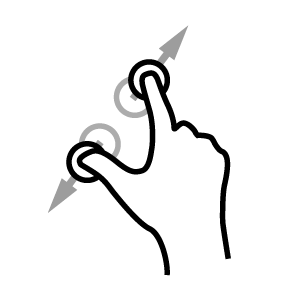
\includegraphics{./Figures/pinch.png}
	\rule{35em}{0.5pt}
	\caption[Pinch]{Pinching outward to indicate larger}
	\label{fig:Pinch}
\end{figure}

%----------------------------------------------------------------------------------------
%	SUBSECTION 3.3
%----------------------------------------------------------------------------------------

\subsection{Rewards}

People like being rewarded, and knowing there is a reward waiting, users are more likely to be motivated to perform well. It doesn't matter that much what the reward is, as long as the user knows that some kind of reward awaits them should they perform well. By tracking data such as time spent on each question and what types of questions or tasks the user successfully answers/completes, we can award players with achievements and badges based on this.

The achievements can be divided into two types: long-term achievements and per-game awards. Long-term achievements can be listed in a "hall of fame" with the names of the players who received them, which will give well-performing players recognition from future players. Examples of such achievements can be scoring above a certain threshold or completing a certain amount of levels/rounds, gaining perfect scores or correct answers on all questions in a certain category, etc.

Per-game awards represent smaller achievements and promote competition between players playing together at the same time. By giving awards to all participating players, we also help players feel included. These small awards should be humoristic, and don't necessarily need to award a positive aspect such as being best, but can "award" players for most incorrect answers or most hits outside their answer box. An example of a popular game that uses this approach is the multiplayer online battle arena game \emph{Heroes of Newerth}\citep{Newerth}. In their \emph{Mid Wars} game mode, a mode much more focused on fun than the competitive aspect, each player will receive two such awards at the end of each game. The awards can be based on a large number of different statistics, such as hero damage or kills, buildings destroyed, gold earned and so on\citep{MidWars}. There are also some number of awards that award feats that may not be particularly impressive, such as having no kills.

%----------------------------------------------------------------------------------------
%	SECTION 4
%----------------------------------------------------------------------------------------

\section{Conducting the Experiments}

This section describes how the experiments will be conducted.
% Chapter 4

\chapter{User Study}

\label{Chapter4}

\lhead{Chapter 4. \emph{User Study}}

%----------------------------------------------------------------------------------------
%	SECTION 1
%----------------------------------------------------------------------------------------

\section{Introduction}

This chapter describes the process for the user study to be performed. It will begin with a description of the user study design, followed by a section on each of the aspects we wish to improve in the existing application: learning, fun and motivation.

%----------------------------------------------------------------------------------------
%	SECTION 2
%----------------------------------------------------------------------------------------

\section{Experiment Design}

The user study will have a between-groups design. The application will be extended with the changes proposed in the previous chapter, resulting in a new version. Users will then be divided into two separate groups: one group will use the old (current) application, while the other will use the new, updated application. Both groups will go through the same procedure (to the extent that this is possible), but using different versions of the application. The groups will consist of subjects of both genders and of varied genders. These subjects will be recruited through the relevant museums and at the university.

The between-groups design allows for a relatively fast user study. The updated application can be implemented to its full extent before testing, and only one round of testing is required. By performing the testing at approximately the same time, it also becomes easier to make sure that subjects in both groups receive the same test with the same coverage, as projects are prone to change over time, which could affect groups tested at vastly different points in time.

%----------------------------------------------------------------------------------------
%	SECTION 3
%----------------------------------------------------------------------------------------

\section{Improved Learning}

To understand whether the changes to the application affect the learning potential of the game, subjects will be presented with a pen-and-paper test before and after using the application. The results from both of these tests will then be compared. The assumption is that subjects will have better results after playing the game. If the updated application provides a better learning environment, the subjects in the new-group should show a bigger improvement in the post-game test from the pre-game test than the old-group.

%----------------------------------------------------------------------------------------
%	SECTION 4
%----------------------------------------------------------------------------------------

\section{Increased Fun and Motivation}

To understand the impact on fun and motivation, we not only need to observe the subjects during play, but ask them about their experience. Additionally, the application will passively gather data during play. This data will show where users touch, and less interesting parts of the application will be less frequently visited. Observations during play will note player reactions and utterances and at what points during play they occur. After they are finished playing, a questionnaire will gauge them on their thoughts on both fun and motivation. Points that should be covered in the questionnaire include the following:
\begin{itemize}
	\item Was the game fun to play?
	\item Which mode was the most fun?
	\item Was the game too easy/too hard?
	\item Would you play the game during a regular visit to the museum?
	\item Did you feel motivated to play?
	\item If you felt motivated, what made you feel motivated?
	\item If you didn't feel motivated, what would have motivated you?
\end{itemize} 
%\chapter{Conclusion}

\label{Chapter5}

\lhead{Chapter 5. \emph{Conclusion}}

%----------------------------------------------------------------------------------------
%	SECTION 1
%----------------------------------------------------------------------------------------

\section{Conclusion}

Throughout the paper we have looked into previous work on edu-games and interactive museum exhibits, game elements and motivation. We have seen that edu-games can be effective tools for learning in informal learning situations and for facilitating attitude change where traditional information channels struggle. We have also seen that finding the right balance between a game and an informational tool can be difficult, and that it is important to realize that the motivations for playing the game in some cases may be the game itself rather than the learning it supports.

We have also seen that large multi-touch displays not only encourage group activities and collaboration, but that large multi-touch exhibits are expected to support interaction from multiple simultaneous users. Furthermore, users find these kind of exhibits fun and easy to interact with, and having several input sources leads to less frustration.

Finally, we have seen that successful games share a lot of common elements, and that motivation stems from three main elements: challenge, fantasy and curiosity. Challenge derives from goals and uncertain outcome, which can be achieved through various means, such as randomness and hidden information. Challenge and goals affect self-esteem, and it is important that they are balanced, e.g. through variable difficulty. While achievements is a very popular game element, it is important that they are implemented in a way that they actually increase motivation rather than function as a detriment, reducing the game to a simple grind for achievements.

Moving forward, the existing application will be extended with additional game modes, variable difficulty levels and randomization to increase the challenge and the fun. Additionally, the players will be motivated to perform their best with new goals: getting in the hall of fame and topping the high scores lists. The extended application will be tested in parallel with the current version by separate groups to compare them on aspects of fun, motivation and learning. Through questionnaires, observations and analysis of background data, we should be able to assess what elements are effective in reaching our goals of a fun, motivating and educational game. 
%\input{Chapters/Chapter6} 
%\input{Chapters/Chapter7} 

%----------------------------------------------------------------------------------------
%	THESIS CONTENT - APPENDICES
%----------------------------------------------------------------------------------------

\addtocontents{toc}{\vspace{2em}} % Add a gap in the Contents, for aesthetics

\appendix % Cue to tell LaTeX that the following 'chapters' are Appendices

% Include the appendices of the thesis as separate files from the Appendices folder
% Uncomment the lines as you write the Appendices

%% Appendix A

\chapter{Appendix Title Here} % Main appendix title

\label{AppendixA} % For referencing this appendix elsewhere, use \ref{AppendixA}

\lhead{Appendix A. \emph{Appendix Title Here}} % This is for the header on each page - perhaps a shortened title

Write your Appendix content here.
%\input{Appendices/AppendixB}
%\input{Appendices/AppendixC}

\addtocontents{toc}{\vspace{2em}} % Add a gap in the Contents, for aesthetics

\backmatter

%----------------------------------------------------------------------------------------
%	BIBLIOGRAPHY
%----------------------------------------------------------------------------------------

\label{Bibliography}

\lhead{\emph{Bibliography}} % Change the page header to say "Bibliography"

\bibliographystyle{unsrtnat} % Use the "unsrtnat" BibTeX style for formatting the Bibliography

\bibliography{Bibliography} % The references (bibliography) information are stored in the file named "Bibliography.bib"

\end{document}  